\begin{question}
Here's a little ditty, about Jack and Diane,
two American kids growing up in the heartland.
The game is below.
% \footnote{Cliff Bekar, Lewis and Clark College}
  \begin{table}[h!]
    \centering
    \setlength{\extrarowheight}{2pt}
    \begin{tabular}{*{5}{c|}}
      \multicolumn{2}{c}{} & \multicolumn{3}{c}{Diane} \\\cline{3-5}
      \multicolumn{1}{c}{} &     & $x$ & $y$ & $z$ \\\cline{2-5}
      \multirow{3}*{Jack}  & $a$ & 1,1 & 2,1 & 2,0 \\\cline{2-5}
                           & $b$ & 2,3 & 0,2 & 2,1 \\\cline{2-5}
                           & $c$ & 2,1 & 1,2 & 3,0 \\\cline{2-5}
    \end{tabular}
  \end{table}
\begin{tasks}
    \task (\points{6}) Find all pure Nash strategy profiles and outcomes
    \textit{if Jack moves first}.
    Carefully detail and explain your strategy profiles.
\end{tasks}
\begin{solution}
  \begin{tasks} 
    % \task Players: $\{ \text{Jack, Diane} \}$
    % Strategy sets: $S_{\text{Jack}} = \{ a, b, c \}$
    % $S_{\text{Diane}} = \{ x, y, z \}$ \\
    % For Jack, $b$ and $c$ are best responses to $x$,
    % $a$ is BR to $y$,  
    % and $c$ is BR to $z$. \\
    % For Diane, $x$ and $y$ are BR to $a$,
    % $x$ is BR to $b$,
    % and $z$ is BR to $c$.  \\
    % There are two strategy profiles where each player's best responses intersect:
    % \begin{itemize}
    %   \item $N_1 = \left( b, x \right)$ results in payoffs (2,3) \\
    %   Jack's strategy is to choose $b$, 
    %   Diane's strategy is to choose $x$.
    %   Neither have regrets about their strategy choice;
    %   given that Jack is choosing $b$, Diane can't get a higher payoff by deviating.
    %   Given that Diane is playing $x$, Jack is indifferent between playing $b$ and $c$ but he can't get a strictly higher payoff by deviating. 
    %   The resulting outcome is that Jack gets $2$, 
    %   Diane gets $3$.
    %   \item $N_2 = \left( a, y \right)$ results in payoffs (2,1) \\
    %   Jack's strategy is $a$, Diane's is $y$. 
    %   When Jack plays $a$, Dianne is indifferent between $x$ and $y$, but
    %   still cannot deviate to a strictly higher payoff.
    %   When Diane plays $y$, Jack's best response is $a$ because $2>\{0,1\}$. 
    %   The outcome is that Jack gets $2$ and Diane gets $1$.
    % \end{itemize}
    % These are the only two \textit{pure strategy} Nash equilibria
    % because there are no other intersections of pure strategy best responses.
    % Note that even though $N_1$ Pareto dominates $N_2$ 
    % (Jack is indifferent; $2=2$, and Diane is better off; $3>1$),
    % there is no \textit{unilateral} deviation that would reach $N_1$
    % from $N_2$.
    \task
    See the extensive form game tree below. \\
    \begin{center}
      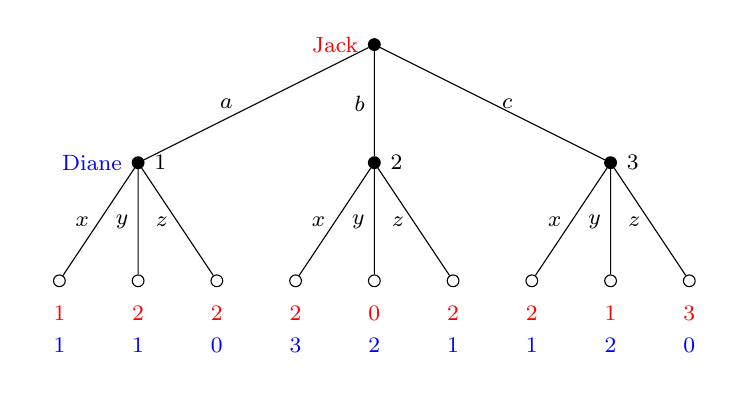
\begin{tikzpicture}[font=\footnotesize]
    \tikzstyle{solid node}=[circle,draw,inner sep=1.5,fill=black]
    \tikzstyle{hollow node}=[circle,draw,inner sep=1.5]
    \tikzstyle{level 1}=[level distance=15mm,sibling distance=3cm]
    \tikzstyle{level 2}=[level distance=15mm,sibling distance=1cm]
    \tikzstyle{level 3}=[level distance=15mm,sibling distance=.5cm]
    
    \node(0)[solid node,label=left:{\color{red} Jack}]{}
        child{node(1)[solid node,label=left:{\color{blue} Diane },label=right:{$1$}]{}
            child{node[hollow node,label=below:{
                \begin{tabular}{c}
                     {\color{red} 1}  \\
                     {\color{blue} \boxed{1}} 
                \end{tabular}
            }]{} edge from parent[] node[left]{$x$}}
            child{node[hollow node,label=below:{
                \begin{tabular}{c}
                  {\color{red} \boxed{2}}  \\
                     {\color{blue} \boxed{1}} 
                \end{tabular}
            }]{} edge from parent node[left]{$y$}}
            child{node[hollow node,label=below:{
                \begin{tabular}{c}
                     {\color{red} 2}  \\
                     {\color{blue} 0} 
                \end{tabular}
            }]{} edge from parent[ ] node[left]{$z$}}
            edge from parent node[left,xshift=-5]{$a$}
        }
        child{node(2)[solid node,label=right:{$2$}]{}
            child{node[hollow node,label=below:{
                \begin{tabular}{c}
                  {\color{red} \boxed{2}}  \\
                     {\color{blue} \boxed{3}} 
                \end{tabular}
            }]{} edge from parent[] node[left]{$x$}}
            child{node[hollow node,label=below:{
                \begin{tabular}{c}
                     {\color{red} 0}  \\
                     {\color{blue} 2} 
                \end{tabular}
            }]{} edge from parent[ ] node[left]{$y$}}
            child{node[hollow node,label=below:{
                \begin{tabular}{c}
                     {\color{red} 2}  \\
                     {\color{blue} 1} 
                \end{tabular}
            }]{} edge from parent[ ] node[left]{$z$}}
            edge from parent node[left]{$b$}
        }
        child{node(3)[solid node,label=right:{$3$}]{}
            child{node[hollow node,label=below:{
                \begin{tabular}{c}
                  {\color{red} \boxed{2}}  \\
                     {\color{blue} 1} 
                \end{tabular}
            }]{} edge from parent[ ] node[left]{$x$}}
            child{node[hollow node,label=below:{
                \begin{tabular}{c}
                     {\color{red} 1}  \\
                     {\color{blue} \boxed{2}} 
                \end{tabular}
            }]{} edge from parent[] node[left]{$y$}}
            child{node[hollow node,label=below:{
                \begin{tabular}{c}
                  {\color{red} \boxed{3}}  \\
                     {\color{blue} 0} 
                \end{tabular}
            }]{} edge from parent[ ] node[left]{$z$}}
            edge from parent node[right]{$c$}
        };
\end{tikzpicture}

    \end{center}
 
    \begin{itemize}

      \item 
      $\mathbf{N_1} = (\mathbf{a}, \ \mathbf{y_1} x_2 x_3 )$ and
      $(\mathbf{a}, \mathbf{y_1}x_2y_3)$
      
      Any set of strategies in which Jack chooses $a$
      and Diane chooses $y$ in node $1$ 
      is a Nash as long as Diane chooses anything other than $z$ in node 3
      results in neither having regrets given the other's strategy.
      Diane will always play $x$ in node 2.

      The payoffs obtained in this equilibrium are $({\color{red} 2}, {\color{blue} 1})$

      \item 
        $\mathbf{N_2} = \left( \mathbf{b}, \ s_1 \mathbf{x_2} s_3 \right) $
      
      where:
      \begin{itemize}
          \item $s_1$ could be $\mathbf{x}$, $\mathbf{y}$; 
          \item $s_3$ could be either $\mathbf{x}$, $\mathbf{y}$, or $\mathbf{z}$.
      \end{itemize}

      Any set of strategies in which Jack chooses $b$,
      Diane is indifferent between $x$ and $y$ at node 1 which is not on the equilibrium path of play,
      and Diane chooses $x_2$ given that jack chooses $b$. 

      The equilibrium outcome of any of these Nash strategy profiles
      would be $({\color{red} 2}, {\color{blue} 3})$

    \end{itemize}

  \end{tasks}


\end{solution}
\end{question}